\documentclass{article}

\begin{document}


In order to train a regression model of the hand kinematics based on EMG signal, we need to provide a ground truth describing the evolution of the hand gesture synchronized with this signal.
	Two kinds of devices are usually used to record this information: a CyberGlove or a camera motion tracking system. 
	
	\subsubsection{CyberGlove}
	
	The CyberGlove made by the company CyberGlove Systems (\url{http://www.cyberglovesystems.com/}) is a motion capture device composed of a glove with multiple strain gauges which capture the motion of the hand. Its latest currently available version, the CyberGlove III, can capture up to 22 joint-angles with a resolution lower than 1 degree. The  CyberGlove II was used for the creation of the Ninapro datasets \cite{ref:ninapro, ref:comp6EMGsetup} and the KIN-MUS UJI Dataset \cite{ref:KinMusUji}.
	
	\begin{figure}[h]
		\centering
		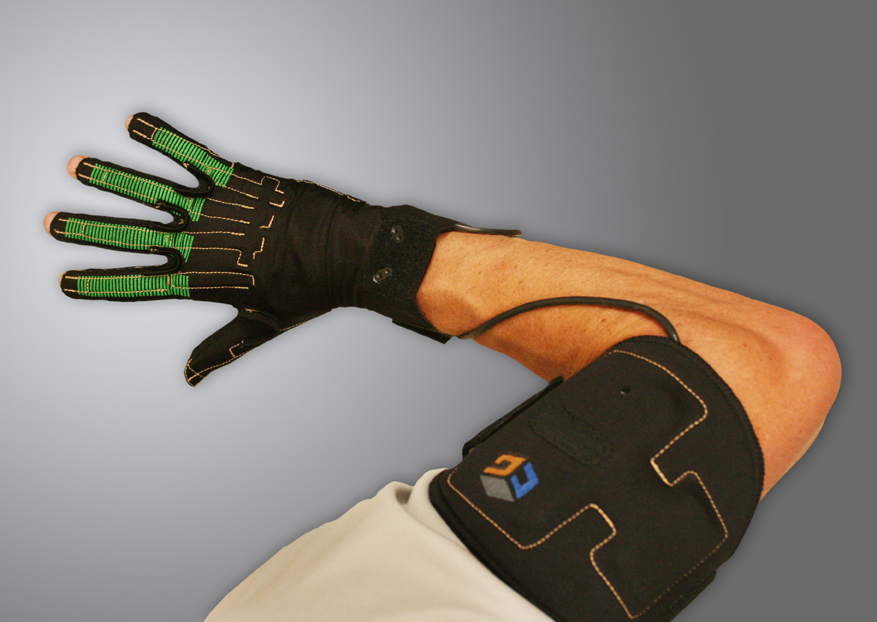
\includegraphics[width=10cm]{images/cyberGlove3.png}
		\caption{Picture of the CyberGlove III from the CyberGlove System website (\url{http://www.cyberglovesystems.com/cyberglove-iii/})}
		\label{fig:cyberGlove3}
	\end{figure}
	
	Even if this device is really easy to use and provides an accurate reconstruction of the hand joint-angles, it does not allow to easily reproduce the data collection experiment as its price can quickly reach several tens of thousands of euros and it is not easily found in every laboratory. Some people have shared instructions on how to build an homemade CyberGlove for 40 dollars \cite{ref:diyCyberGlove} but there is no guarantee on the performance that it can provide.
	
	
	\subsubsection{3D motion camera tracking}
	
	This technique is usually used for cinematographic special effects. It is composed of 2 elements: an ensemble of markers placed on the tracked object (consisting of small white balls) and a set of fixed cameras located around the subject that each film it from a different point of view. The location of each marker in the 3D space can be computed from its position each cameras vision.
	
	To record the finger kinematics, 22 markers need to be placed as shown in the following figure.
	
	\begin{figure}[h]
		\centering
		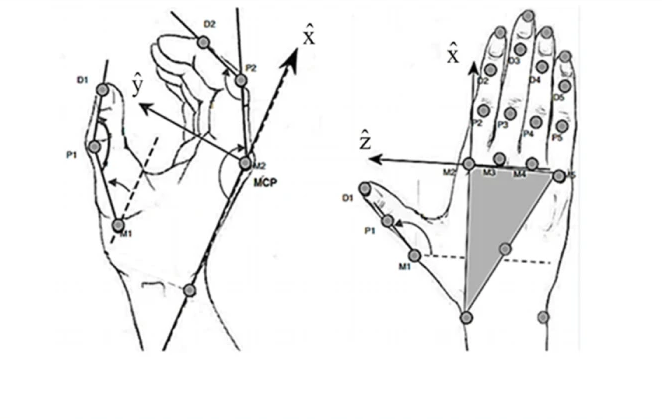
\includegraphics[width=10cm]{images/motionCaptureMarker.png}
		\caption{Positions of the 22 markers used to track the fingers kinematics \cite{ref:Ngeo2014}}
		\label{fig:cyberGlove3}
	\end{figure}
	
	This device has a precision of less than 0.5mm \cite{ref:Ngeo2014}. However, some study say that it is not reliable enough for finger tracking as their movement is too precise \cite{ref:KinMusUji}.
	
	
\end{document}